


\section{Robothanden}
FÖRKLARA FRIHETSGRADER? = Frihetsgrader beskriver hur många oberoende variabler som behövs för att entydigt ange läget för ett system.
I detta avsnitt presenteras en överblick över de komponenter som utgör den mekaniska handen.  %%Meccano™ använts som grund vilket har både fördelar och nackdelar jämfört med att bygga alla delar från början. Eftersom konstruktionen innehåller flera delar vars inbördes passform påverkar hur väl rörelser fungerar måste tillverkningen av delarna utföras med god noggrannhet. Meccanos standardbyggsats innehåller flera olika standardiserade delar som enkelt kan monteras i flera olika kombinationer.Delarna anses även ha tillräcklig noggrannhet för att slutprodukten ska kunna utföra de uppsatta målen. Eftersom konstruktionen av handen går snabbare med färdiga delar kan mer fokus läggas på den mer resurskrävande elektroniken. Nackdelen är att konstruktionen blir begränsad till att endast kunna tillverkas av tillgängliga komponenter, men detta kringgås med konstruktion av enstaka kritiska komponenter.%%
Handen består av två fingrar och en tumme som beskrivs utförligare i sina respektive avsnitt. På fingrar och tumme sitter det även plastskal som har som uppgift att skapa bättre greppytor. Handen har tillverkats av Meccano för att underlätta tillverkning. 


Handens utformning är en funktion av hur fingrarna önskas vara positionerade relativt varandra och detta utprovades i CAD-miljö utefter förmågan att utföra ett antal önskade grepp. Handen har även tillräckligt stor yta för att möjliggöra integrering av aktuatorer, kontrollenhet och strömförsörjning i en enda enhet. I figuren ovan syns från vänster till höger syns de utprovade greppen.



\subsection{Fingrar och tumme}
Med utgångspunkten mänsklig motorik designades handens två identiska fingrar för att få ett människolikt rörelsemönster.


\begin{figure}[H]
\includegraphics[height=0.35\textheight]{img/fingerbild}
\caption{Översiktsbild fingerdesign.}
\end{figure}

Fingrarna har tre leder varav Led 1 och Led 2 är separat kontrollerbara. Led 3 är via ett stag tvångsstyrd av Led 2 för att imitera hur ett mänskligt finger beter sig när handen sluts. Jämfört med det mänskliga fingret saknas en frihetsgrad i Led 1 för vridning av fingret i sidled. En fördel med två separat kontrollerbara leder är att fingrarnas rörelseomfång och funktionella förmåga utökas.

\begin{figure}[H]
Bild tumme

\caption{Beskrivning}
\end{figure} Tummen har endast två separata frihetsgrader och sitter fast positionerad i handen för att kunna utföra ett pincettgrepp med finger 1. Detta är tillräckligt för att uppnå målen, men jämfört med den mänskliga tummen som kan möta samtliga fingertoppar är detta ett stelt utförande.
%\begin{minipage}[t]{0.5\textwidth}
%\begin{figure}[H]
%\includegraphics[width=0.57\textwidth]{img/rorelse1}
%\caption{En kontrollerbar frihetsgrad.}
%\end{figure}
%\end{minipage}
%\begin{minipage}[t]{0.5\textwidth}
%\begin{figure}[H]
%\includegraphics[width=0.5\textwidth]{img/rorelseomfang}
%\caption{Två kontrollerbara frihetsgrader.}
%\end{figure}
%\end{minipage}

\subsection{Fingertoppar och sensorer}
BILD PÅ SENSORER, FINGERTOPPAR MED GUMMI och sensor PÅ(sprängskiss) 
\begin{figure}[H]
X
\label{fig:sensor}
\caption{Beskrivning}
\end{figure}
För att reglera hur hårt man trycker sitter det tre trycksensorer längst ut på varje fingertopp. Se \ref{fig:sensor}. Fingertopparna är formade för att ge ett bra pincettgrepp där sensorerna registrerar hur hårt objektet greppas. (Fingertopparna är utskriva i plast med en 3D-skrivare?) Sensorerna är av modell FSR-400 och kan registrera normaltryck i spannet 0.11-110 MPa. Trycksensorn ändrar resistans vid kompression och ett värde avläses i mikrokontrollen för reglering, där jämförs värdet med det kalibrerade värden från tester ( SE APP KALIBRERING AV SENSORER) för att säkerställa att handen griper med rätt tryck(KRAFT??). Över sensorn sitter ett 3 mm tjockt lager av syntetiskt gummi för att skydda sensorns samt ge större friktion vid hantering av objekt. Nedre delen av fingertoppen fungerar som stöd vid grepp men där mäts inte kontakttrycket. 
\section{Aktuering}
Total har handen åtta frihetsgrader varav sex är separat aktuerbara. I detta avsnitt presenteras aktuatorer och kraftöverföring.
\subsection{Servon}
\begin{figure}[H]
\includegraphics[height=0.2\textheight]{img/servo}
\caption{Blue Bird BMS-660DMG+HS servo.}
\label{fig:servo}
\end{figure}
Aktuatorer för samtliga leder är Blue Bird BMS-660DMG+HS. Se figur~\ref{fig:servo}. Dessa servon används för att de uppfyllde kraven på vridmoment med god marginal (se APPENDIX A.HIYTF för dimensionerande beräkningar). Vid en matningsspänningen på 6 Volt har servot ett maximalt vridmoment på 1.42 Nm och en högsta rotationshastighet på 6.16 rad/s vid obelastat läge. Servona har ett totalt rörelseomfång på 120 grader vilket är standard för hobbyservos. Servona regleras via PWM-signaler och har en intern positionsreglering, detta gör att servona alltid arbetar för att nå det önskade läget och återgår till detta läge efter en eventuell störning.

\subsection{Kraftöverföring}
\begin{figure}[H]
BILD PÅ STAG, BILD PÅ SENA MED HJUL

\caption{Beskrivning}
\end{figure}
Led 1 i samtliga fingrar aktueras via stag, vilket gör att de kan föras fram och tillbaka av respektive servo. För att aktuera Led 2 i samtliga fingrar används en sena. Senan utgörs av en fiskelina dimensionerad för en dragkraft på 330 N. Största dragkraften i senan uppstår då servo arbetar vid maximalt vridmoment och uppgår till 118 N med 12 mm servohorn. För att återföra fingret till sitt räta läge används en vridfjäder som sitter runt led 2.

\section{Reglerhandsken}
\begin{figure}[H]
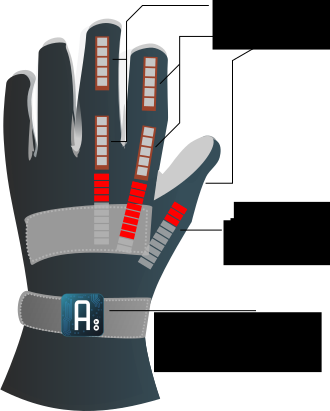
\includegraphics[height=0.5\textheight]{img/kontrollhandske}
\caption{Beskrivning}
\end{figure}
För att reglera robothanden används en reglerhandske som användaren har på sin hand, detta ger en intuitivt reglering (se figur). På tumme, pekfinger och långfinger på handsken sitter två flexsensorer var som följer användarens hand och ändrar resistans beroende på hur mycket de böjs. Denna resistansförändring använder man som insignal till mikrokontrollen som sitter på reglerhandsken, som i sin tur skickar styrsignaler till mikrokontrollen på robothanden. Se \ref{sec:mikro}. 

Handsken är gjord av textil och flexsensorerna är insydda i små påsar som underlättar montering av sensorerna på handsken. (Se figur)
(Bild på handsken)  
\section{Trådlös kommunikation}
\section{Signalbehandling}
\section{Mikrokontroller}
\label{sec:mikro}
info om våra microcontroller. Bluetooth moduelerna och hur det programmerats samt hur det fungerar.
\section{Elektriska kretsar}
\begin{figure}[H]
\includegraphics[height=0.5\textheight]{img/schemahandske}
\caption{Kopplingsschema för styr/regler-handsken.}
\end{figure}

Dedssa kretsar har byggts och lötts på kretskort- 

\section{Algoritmer}
Här presenteras de styralgortimter som bestämmer hur handen beter sig när den följer användarens input samt identifierar och greppar objekt. 
\subsection{Objektidentifiering}
\begin{figure}[H]
EN BILD SOM FÖRKLARAR DETTA, SAMT VILKA OBJEKT VI VALT ATT identifierar och hur vi gör det...
\caption{Beskrivning}
\end{figure}
Antaganden: Servona står i önskat läge, det vill säga tidsfördröjningen som uppstår då servona skall vrida sig från godtycklig position till den önskade antags vara så liten vid normalt användande att den kan försummas. Då ingen mätning av servonas verkliga position görs, är den enda informationen om fingrarnas lägen det önskade servoläget. 

FIXA FLÖDESSSCHEMA OCH ETT ARDUINO PROGRAM Känner av tryck (över visst gränsvärde) på tumme och motstående finger->, lagrar användarens input läge då detta inträffar ( för att när användaren går utanför detta igen (öppnar sin hand) så skall handen återgår till att följa användaren) -> beräknar avståndet mellan sensorerna-> checkar av avståndet mot en lista av fördefinerade objekt som innehåller , storlek och önskat trycksensorvärde med en +/-tolerans för att inte handen ska stå och flippa som en tok för att uppnå EXAKT rätt värde-> TADAA!!-> när användaren öppnar sina fingrar utanför "kontaktläget" följer handen efter igen...
Mer teksti


